\section{Rekombinacija}
\label{app:beta}

\begin{figure}[h]
\centering
	\subfloat[$\alpha d = 10$ su difuzija]{
		\label{fig:beta:1}
		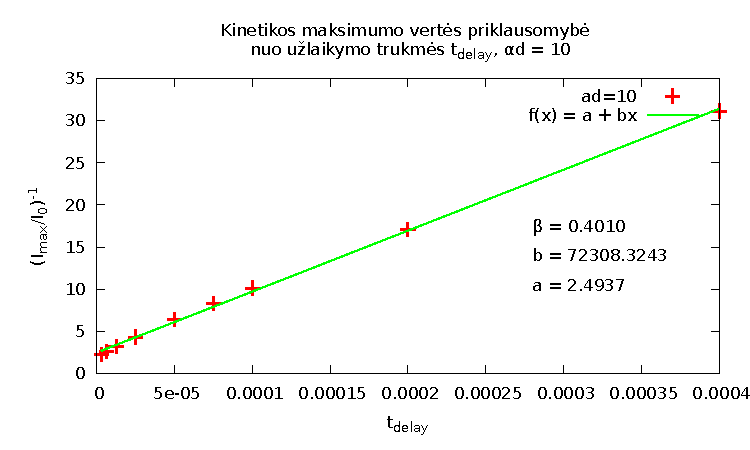
\includegraphics[width=0.5\textwidth]{./media/pdf/invert_ad10_recomb_diff.pdf}
	}
	\subfloat[$\alpha d = 10$ be difuzijos]{
		\label{fig:beta:2}
		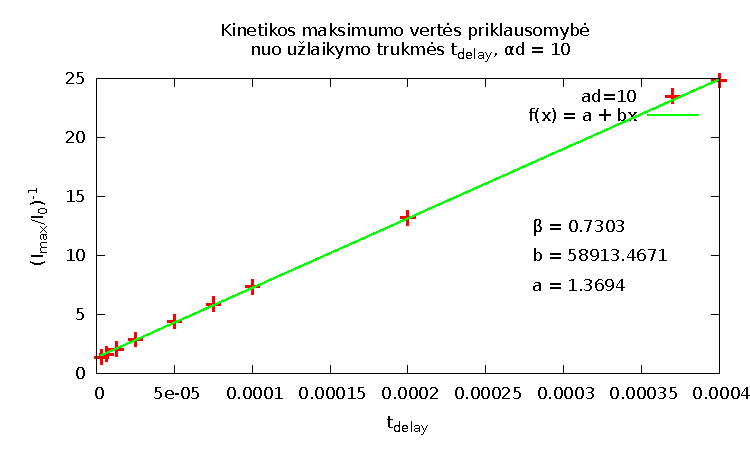
\includegraphics[width=0.5\textwidth]{./media/pdf/invert_ad10_recomb_nodiff.pdf}
	}\\
	\subfloat[$\alpha d = 0.1$ su difuzija]{
		\label{fig:beta:3}
		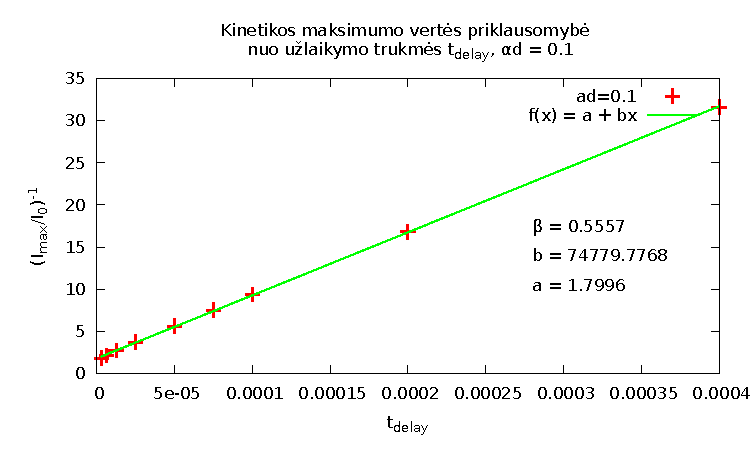
\includegraphics[width=0.5\textwidth]{./media/pdf/invert_ad01_recomb_diff.pdf}
	}
	\subfloat[$\alpha d = 0.1$ be difuzijos]{
		\label{fig:beta:4}
		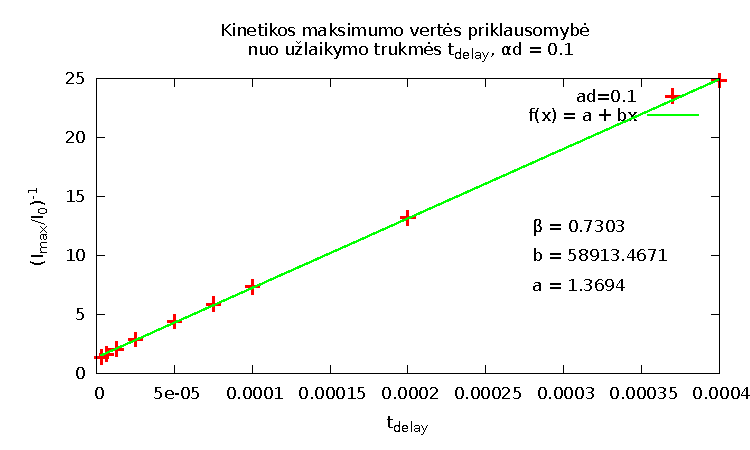
\includegraphics[width=0.5\textwidth]{./media/pdf/invert_ad01_recomb_nodiff.pdf}
	}
\caption{Įvairūs bandymai skaičiuoti rekombinacijos koeficientą.}
\end{figure}